\section{Subdomain decomposition}

The results show that the MPI implementation does not improve processing-time performance with respect to the reference parallel implementation. The reasons for this behavior become apparent in the graphical results in two main ways.

First, the temporal distribution of the execution clearly shows that the time associated with communication and synchronization between subdomains becomes a dominant component of the overall dynamics of the system, even when the number of planets in the galaxy is as low as 1000. As the domain is subdivided, the processes must exchange more information and remain synchronized at the boundaries of their local regions, which introduces an overhead that can outweigh the benefits of distributing the computation. This growth in communication and synchronization costs explains an important part of the observed performance degradation.

Second, the computation time itself does not exhibit a significant improvement, and this is directly related to the way the workload is distributed according to the calculation density in the different subdomains. Since the total execution time is determined by the slowest process, the overall behavior of the system deteriorates when the global domain is divided into static subdomains that do not take into account the nonuniform distribution of computational work. In other words, some processes are assigned regions with a much higher computational density than others, which generates load imbalance and forces the rest of the system to wait. As a consequence, the potential benefit of parallelization is reduced not only by communication overhead, but also by the fact that the static partitioning strategy fails to adapt to the heterogeneous structure of the problem.


\begin{figure}[htbp]
\centering
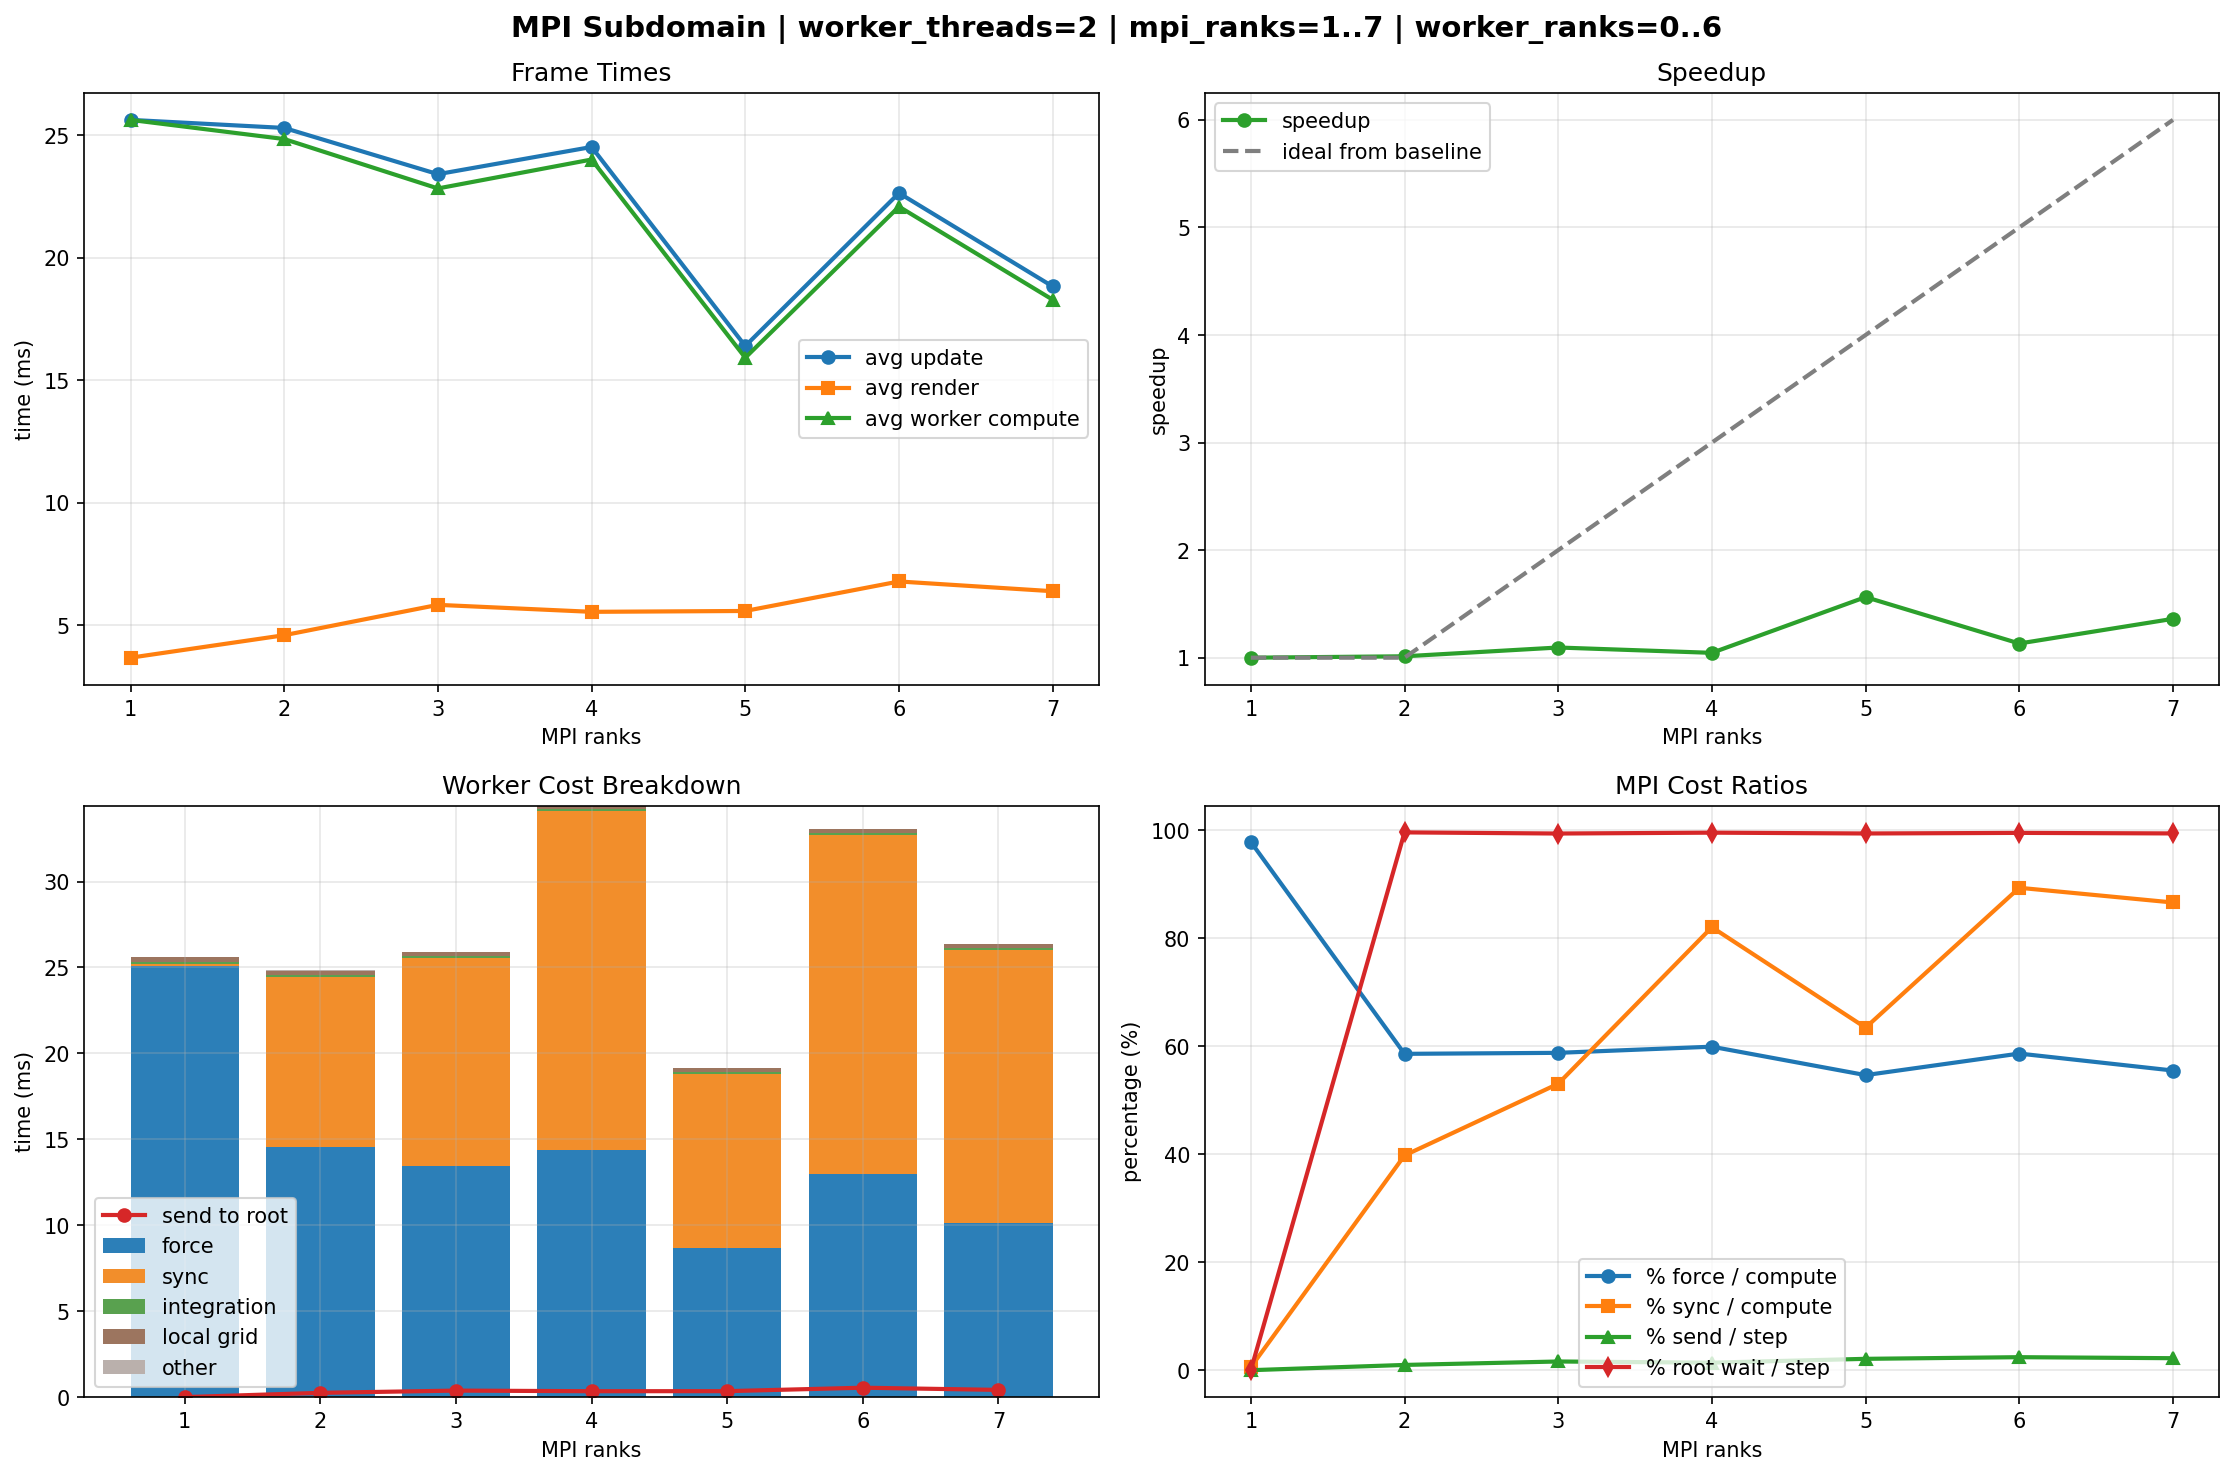
\includegraphics[width=0.82\linewidth]{images/mpi_subdomain_timings.png}
\caption{Mesures de performance de la version MPI par sous-domaines.}
\label{fig:mpi_subdomain_timings}
\end{figure}

\subsection{Distribution de densité}
Le fait que la distribution de la densité ne soit pas uniforme dans le domaine engendre un effet de déséquilibre dans la répartition des charges entre les différents sous-domaines qui sont implémentés. Cela a, à son tour, pour conséquence que certains processus prennent un temps de calcul plus élevé que les autres et, par conséquent, affectent la performance générale du système face à la parallélisation, compte tenu des conditions de charge auxquelles ils sont soumis. C’est pour cette raison qu’il est proposé, comme option alternative à une distribution dans un domaine cartésien 2D avec une répartition équitable et des sous-domaines de taille équivalente, d’implémenter une distribution en sous-domaines dont les dimensions ne soient pas nécessairement uniformes dans le domaine global, mais qu’elles s’adaptent plutôt aux particularités des conditions de charge, de manière à obtenir une distribution permettant d’avoir moins de cellules par processus dans la zone centrale du domaine global, puisque c’est là que la charge se concentre, et davantage de cellules par processus dans les autres zones. Le problème associé à cette implémentation est que la division des sous-domaines en sous-domaines incorporant un plus petit nombre de cellules par processus implique également un besoin plus important de communication dans la résolution des conditions de frontière entre les différents sous-domaines, ce qui s’accentuerait encore davantage dans la zone de plus forte densité, pouvant ainsi avoir un effet contre-productif sur les temps d’exécution.
